\chapter{Introdução}
\label{cap-introducao}

\section{Contexto}
\label{section:contexto}

Menos de 1\% das empresas do Brasil conseguem manter uma taxa de crescimento acima dos 20\% anuais por um período de três anos consecutivos, como demonstrado pela \citeonline{indiceglobaldoempreendedorismo}. As mesmas também foram responsáveis por mais de 40\% dos novos empregos gerados no país e, em média, cerca de 100x mais empregos do que as empresas tradicionais. Tais empresas com altos índices de crescimento são conhecidas como ``\textit{scaleups}'' e recebem cada vez mais atenção pelo seu grande impacto. O foco deste trabalho será em torno das ``\textit{startups}'', como são conhecidas as ``\textit{scaleups}'' da área de tecnologia da informação em busca de modelos de negócios inovadores e escaláveis.

\citeonline{Graham2012} defende que o único fator essencial para que uma organização seja classificada como \textit{startup} é o seu crescimento, para ele qualquer outro fator nada mais é do que um reflexo deste. Idealmente Graham defende que \textit{startups} precisam crescer entre 5 e 7\% por semana e que qualquer indicador acima de 10\% seria algo excepcional. Para \citeonline{Sutton2000} a característica mais básica de uma \textit{startup} é ser nova e inexperiente quando comparada com organizações estabelecidas e maduras, ele também as caracteriza como organizações que trabalham com poucos recursos e geralmente acompanham novas tendências de tecnologia e mercado, além de altamente sensíveis à diversos fatores influenciadores (investidores, clientes, parceiros e concorrentes).

Uma \textit{startup} também pode ser vista como uma instituição humana projetada para criar novos produtos e serviços sob condições de extrema incerteza, como definiu \citeonline{Ries2011}. Para ele o objetivo de uma \textit{startup} é descobrir qual o produto certo que os consumidores queiram e estejam dispostos a comprar, e/ou usar, o mais rápido possível. \citeonline{isenberg2016} identificou em pesquisa que a maior parte das pessoas entrevistadas associavam o termo como referência a empresas de tecnologia como o ``Snapchat'' ou o ``WhatsApp''.

Para construir produtos tecnologicamente inovadores geralmente elas precisam utilizar novas tecnologias, ferramentas e técnicas de gestão e desenvolvimento, como observado por \citeonline{Paternoster2014}. Esse cenário condiz com o mapeamento realizado por \citeonline{Polovets2014}, o qual constatou que a maior parte das \textit{startups} analisadas utilizam tecnologias como \textit{Javascript}, \textit{Node.js}, \textit{Ruby}, \textit{Ruby on Rails}, \textit{Python} e \textit{HTML5} e hospedam seus \textit{softwares} em grandes infraestruturas escaláveis como \textit{Amazon Web Services} e \textit{Heroku}. 

No contexto brasileiro, \citeonline{Brinded2015} relata que o país é o terceiro com o maior número de empreendedores do mundo, correspondendo a cerca de 13,8\% da população. Para \citeonline{Acs2016} um dos destaques do Brasil em comparação ao restante do mundo é a percepção de oportunidade.

Nessa linha, governos das três esferas brasileiras (Federal, Estaduais e Municipais) buscam desenvolver políticas públicas de fomento e suporte aos seus ecossistemas empreendedores afim de atrair investimentos, gerar empregos e aumentar a arrecadação de impostos. Alguns dos exemplos de políticas públicas do governo federal com foco em \textit{startups} são os programas Inovativa Brasil, \textit{Startup} Brasil e Fundo Criatec. Em escala estadual, uma boa referência de programa governamental é o ``SEED - \textit{startups} and Entrepreneurship Ecossystem Development'', criado pelo governo de Minas Gerais. Também há diversos casos de governos estaduais e municipais explorando verbas para fomento de tecnologia e inovação de Fundações de Apoio à Pesquisa para oferecer subvenção econômica para \textit{startups}. Além de investimento, alguns projetos de lei como a Lei da Inovação e o Marco Legal da Ciência, Tecnologia e Inovação busca trazer flexibilidade para o ambiente regulatório do Brasil com o objetivo de aumentar as chances de sucesso e crescimento dessas pequenas empresas inovadoras. Do lado privado e da sociedade civil organizada instituições como Endeavor\footnote{https://www.endeavor.org.br/} e Dínamo\footnote{http://www.dinamo.org.br/} buscam atuar de forma a apoiar e colaborar com governos nos processos de regulamentação e fomento aos setores empreendedores.

Especificamente no Distrito Federal, o estado vive um momento de crescimento de atividades no ecossistema de \textit{startups} local, embora o país e a cidade estejam passando por recessão e crises política e econômica o cenário é favorável e a realização de grandes eventos como o \textit{AgileBrazil}, a \textit{World Conference on International Telecommunications}, a \textit{Campus Party} e diversos outros menores organizados pela comunidade local, como meetups e o evento Capital Empreendedora, podem ser vistos como um sinal de que o público brasiliense enxerga o empreendedorismo e a tecnologia como caminhos a serem perseguidos, a atual crise econômica e a ausência de concursos públicos também podem fortalecer esse movimento.

A nível nacional, \citeonline{Mattos2017} aponta o Distrito Federal como o sétimo estado com o maior número de \textit{startups} do país e o segundo com a maior densidade (relação entre número de \textit{startups} por habitantes). Na premiação do ``\textit{Startup} Awards 2017'', evento promovido pela Associação Brasileira de \textit{startups} (AB\textit{startups}) com o objetivo de prestigiar os maiores destaques do ano no cenário brasileiro de \textit{startups}, a universidade do DF UniCeub foi indicada para o prêmio de ``Melhor Universidade'' e o ``Cerrado Valley'', como alguns se referem ao ecossistema de \textit{startups} do Distrito Federal, como melhor comunidade. 

Os últimos dois anos também foram marcados pelo crescimento do interesse de diversas instituições de ensino superior em desenvolver competências empreendedoras em seus estudantes, o surgimento de novas aceleradoras de \textit{startups} (Acceleratus, Cotidiano, Runpal e Unicórnio), novos espaços de \textit{coworking}, incluindo um com foco específico para desenvolvedores de jogos eletrônicos independentes, e eventos (\textit{meetups}) na cidade com a presença de investidores e representantes de fundos de investimento em busca de oportunidades. 

\section{Justificativa}
\label{section:justificativa}

Uma maior quantidade de trabalhos acadêmicos com foco no cenário de \textit{startups} são necessários para apoiar tais atividades e guiar as ações de diversos atores que compõem um ecossistema, como empreendedores, agentes públicos, investidores e acadêmicos, como apontado por \citeonline{Paternoster2014}.

Com base em uma análise das principais publicações acerca do tema nos últimos 300 anos \citeonline{Filion1998} divide o progresso dos estudos acerca do empreendedorismo em cinco períodos representados pela Tabela \ref{table:tendencias_nas_publicacoes_acerca_do_empreendedorismo}.

\begin{table}[!htb]
	\centering
	\begin{tabular}{ | p{6cm} | p{6cm} | p{3cm} | }
		\hline
		\textbf{Tema} & \textbf{Perspectiva} & \textbf{Período} \\ \hline
		O que fazem os empreendedores & Econômica & 1700 - 1950 \\ \hline
		Quem são os empreendedores & Comportamental & 1960 - 1980 \\ \hline
		O que fazem os empreendedores & Administrativa(finanças, marketing, operações, recursos humanos) & 1980 - Atual \\ \hline
		Quais tipos de suporte são necessários para empreendedores & Ciências Sociais(incluindo economia, geográfia e sociologia) & 1985 - Atual \\ \hline
		O que são atividades empreendedoras e quais Competências são necessárias & Empreendedorismo & 1990 - Atual \\ \hline
	\end{tabular}
	\caption{Tendências nas publicações acerca do Empreendedorismo}
	\label{table:tendencias_nas_publicacoes_acerca_do_empreendedorismo}
\end{table}

Embora Filion tenha relatado que até meados da década de 90 pouco se explorou sobre ecossistemas empreendedores, \citeonline{Cukier2016}  demonstraram que nos últimos sete anos houve um crescimento superior a 1000\% na quantidade de artigos acadêmicos indexados pela plataforma Google Scholar com o termo ``\textit{Startup Ecosystems}'', resultado explicitado na Figura \ref{figure:papers_about_startup_ecosystems}.

\begin{figure}[!htb]
	\centering
	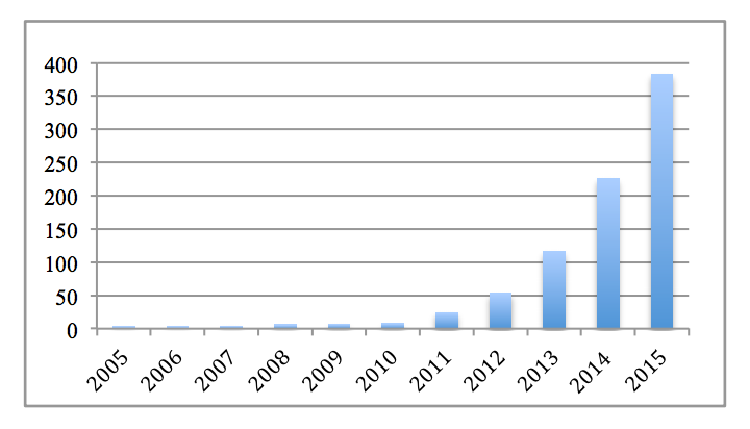
\includegraphics[width=11cm,angle=0]{figuras/papers_about_startup_ecosystems}
	\caption{Frequência do termo ``\textit{Startup Ecosystem}'' no Google Scholar}
	\label{figure:papers_about_startup_ecosystems}
\end{figure}

\citeonline{Unterkalmsteiner2016} apontam a importância de pesquisas que busquem responder questões que envolvam os elementos chaves de um ecossistema frutífero, os tipos de ecossistemas, como eles evoluem e técnicas de avaliação e mensuração de qualidade. \citeonline{Lemos2011} enfatiza que faltam teorias consolidadas sobre as relações entre os diversos elementos que compõem um ecossistema.

Portanto, nota-se que é crescente a demanda por estudos sobre ecossistemas de \textit{startups} e como os diversos fatores que os compõem interagem entre si e impactam o seu desenvolvimento. Até o momento há poucos dados e estudos disponíveis sobre o setor e no atual momento do ecossistema de \textit{startups} do Distrito Federal é relevante que sejam estudadas sua maturidade, a relação entre seus atores, quem são os empreendedores, onde estão e quais os seus desafios, quais os pontos fortes e os pontos de melhora do ecossistema, etc. para que os atores engajados em fomentar o ecossistema (empreendedores, sociedade civil organizada, entidades representativas, academia, governo, etc.) possuam insumos para suas tomadas de decisão. 

\section{Objetivos}
\label{section:objetivo_geral}

Este trabalho consiste em um estudo de caráter exploratório em torno do ecossistema de \textit{startups} de tecnologia do Distrito Federal com o objetivo específico de desenvolver um entendimento acerca do seu desenvolvimento e para que seja feita uma avaliação do seu atual momento e sua maturidade utilizando a metodologia de avaliação de ecossistemas proposta por \citeonline{Kon2014}. 

\section{Organização do Trabalho}
\label{section:organizacao_do_trabalho}

Além desta introdução, este trabalho está organizado em cinco capítulos como descrito a seguir.

O Capítulo \ref{cap-sobre-a-proposta-e-a-metodologia} explora o cenário de pesquisa em torno de ecossistemas de \textit{startups}, o capítulo \ref{cap-metodologia} descreve a metodologia que será aplicada no ecossistema estudado, principalmente no que tange os indicadores utilizados para mensurar sua maturidade.

O Capítulo \ref{cap-resultados} apresenta os resultados obtidos, o que foi constatado, qual a visão dos empreendedores entrevistados e quais ações podem ser tomadas para que o ecossistema do Distrito Federal evolua. Por fim, no Capítulo \ref{cap-conclusoes} é feito um apanhado de tudo o que foi explorado nos capítulos anteriores e o que foi aprendido com o desenvolvimento deste trabalho. Em seguida são apresentados os Anexos e Apêndices do trabalho.
